\documentclass[conference,10pt,letterpaper]{IEEEtran}
%\documentclass[journal,10pt,draftclsnofoot,onecolumn]{IEEEtran}
\usepackage{cite}
\usepackage{graphicx}
\usepackage{amsmath}
\usepackage{multirow}
%\usepackage[ruled,lined,boxed,commentsnumbered]{algorithm2e}
%\usepackage{algpseudocode}
%\usepackage{algorithm}
\usepackage[ruled,vlined,linesnumbered]{algorithm2e}
\usepackage{algorithmic}
\usepackage{amssymb}
\usepackage{subfigure}		
\usepackage{mathtools}
\usepackage[utf8]{inputenc}
\usepackage[english]{babel}
\DeclareMathSizes{10}{8}{8}{8}
\usepackage{color,soul} 
\usepackage{mathptm}
%\usepackage{flushend}
\usepackage{xcolor,pifont}
\newcommand*\colourcheck[1]{%
  \expandafter\newcommand\csname #1check\endcsname{\textcolor{#1}{\ding{52}}}%
}
\colourcheck{blue}
\colourcheck{green}
\colourcheck{red}

\newcommand*\colourx[1]{%
  \expandafter\newcommand\csname #1x\endcsname{\textcolor{#1}{\ding{54}}}%
}
\colourx{red}

\usepackage{pgfplots}
\usepackage{tikz}
\usepackage{float}

\begin{document}

\title{SAT-attack Resilient Sequential Locking}
%\author{\IEEEauthorblockN{
%                    Seetal Potluri,
%		    Akash Kumar}
%                    \IEEEauthorblockA{Chair for Processor Design, \\
%                                      Technical University of Dresden, 01609 Dresden, Germany}}
    

\maketitle
\thispagestyle{empty}

\pagestyle{empty}

\begin{abstract}
SAT-attack is known to decrypt a {\em functionally correct key} of an encrypted combinational circuit. 
Recently, sequential locking was proposed as a defense to SAT-attack on sequential circuits and subsequently ScanSAT was proposed as an unlocking mechanism for the same. 
ScanSAT method converts the sequential locking problem to an instance of logic locking problem, and thereby decrypts the entire sequential key using SAT-attack. 
In this paper, we show that ScanSAT does not guarantee decryption of {\em functionally correct key}, and a defense against ScanSAT.  
%in the presence of encrypted XOR-chains at combinational outputs. Additionally, we propose a low-overhead defense against ScanSAT, that exploits this property. 
The proposed defense had $95-100\%$ success rate when tested on sequentialized ISCAS'85 and MCNC benchmarks, across five different encryption schemes, and $1-3$ orders of magnitude increase in decryption time for large circuits. \\

%Firstly, we provide two different output paths for each observe flip-flop: an XOR/XNOR-type encrypted scan path and an unencrypted functional path. 
%Secondly, we perform XOR/XNOR-type encryption of timing-uncritical combinational outputs, such that they daisy-chain with the encrypted scan chains, to form encrypted XOR/XNOR-chains, making it impossible for the SAT solver to distinguish {\em functionally correct keys} amidst the large equivalence class of {\em scan-mode correct keys}. 
%We propose a new sequential locking scheme, where the flip-flop has an encrypted scan path and an unencrypted functional path, along with encryption key gates only at the combinational outputs. 
%In the presence of proposed sequential locking scheme, applying ScanSAT on $20$ benchmark circuits, across five different state-of-the-art logic-encryption schemes, revealed $95-100\%$ success in decrypting a {\em functionally incorrect key}. Additionally, since encryption is only at the boundary, it is area-efficient and functional output quality evaluation can be executed at RTL-level, making it very efficient and feasible for industry practice. 
%Additionally, the proposed technique incurs minimum timing and energy overheads on the chip's functional mode of operation. 
\end{abstract}

%\noindent {\bf Keywords: } ; 

\section{Introduction}
\label{sec:introduction}
\noindent 
%The fabless fabrication stragies were originally invented by Xilinx co-founder Bernie Vonderschmitt in 1993. 
%Since then, many companies have adopted them to improve their economies of scale, amidst the growing economic demands of maintaining independent foundry in a scaled technology. 
Today, fabless model is the most economical and hence the preferred business model of the semiconductor industry. 
However, IC counterfeiting, piracy and overbuilding in the untrusted offshore foundry have caused major concerns in electronic and defense industries~\cite{pecht06, trimberger07, farinaz:epic}. 

Logic encryption uses a low-overhead combinational chip-locking system, to combat these issues~\cite{farinaz:epic}. 
Several logic encryption have been proposed so far in literature~\cite{farinaz:epic, jv:dac12, jv:tc15, dupuis:iolts14, baumgarten:dandt10}, and each of them have their own merits and demerits. 
The SAT-attack~\cite{pramod:host15} is shown to successfully decrypt the logic encryption keys in all above cases, with over $95 \%$ success rate. 
Recently, sequential locking~\cite{rajit:encryptFF} was proposed as a defense to SAT-attack on sequential circuits. 
The flip-flop encryption is done in this paper, by inserting an XOR gate right at the output of selected flip-flops. 

A major limitation of this technique is that $58-100\%$ of flip-flops were encrypted, which 
induces huge are overhead in real designs. Apart from that, the most recently proposed ScanSAT method~\cite{lilas:aspdac19} 
converts the sequential locking problem to an instance of logic locking problem, and thereby decrypts a {\em functionally correct key} using SAT-attack. 
Thus, it is imperative to come up with a new sequential locking scheme that is area-efficient, as well as, and more importantly resilient to the SAT-attack. 

In this paper, we propose a sequential locking scheme that addresses the aforementioned challenges. The main contributions of this paper are as follows:
\begin{enumerate}
\item We show that ScanSAT does not guarantee decryption of {\em functionally correct key}, in the presence of encrypted XOR-chains at combinational outputs; 
\item We show there is $100\%$ correlation between failure of ScanSAT and presence of encrypted XOR-chains at combinational outputs; 
\item Exploiting this property as a defense mechanism, we propose a new low-overhead encrypted scan cell, that consists of an unencrypted functional path and an encrypted scan path; 
\item Finally, to increase the success rate of successful functional corruption, we propose an iterative combinational key gate pushing algorithm, that makes the sequential circuit resilient to SAT-attack. 
\end{enumerate}


\section{Attack model}
\noindent The attack model used in this paper is same as the one used in~\cite{pramod:host15}. More specfically, we consider a malicious foundry, where the attacker 
has access to layout and mask information. Hence, the gate-level netlist can be reverse-engineering from this. We also assume that the attacker has access to an activated
IC on which to apply input patterns and observe outputs. This could be obtained by purchasing an activated IC from the open
market. The components of our attack model are therefore: (i) a gate-level netlist of the encrypted IC and (ii) a means for applying arbitrary input patterns and observing the resultant
outputs on an activated IC.

\section{Access model}

\noindent Since the SAT-attacker needs access to every flip-flop in the IC, this can be achieved by operating the IC in scan mode of operation by asserting the test mode signal. In today's SoCs, it is only possible to access the scan architecture through embedded deterministic test (EDT) architecture, the on-chip decompression/compression scheme, which also comes with a bypass mode for debug purposes. Moreover, the SAT-attacker wants to apply very specific values to these flip-flops to force the logic nodes to specific states and capture the exact responses, in order to decrypt one of the correct keys. This is possible only in the EDT-Bypass mode. In summary, the access model is (i) initializing flip-flops during scan shift; and (ii) using EDT bypass mode to have direct access to scan-chains. 

\begin{figure}
\centering
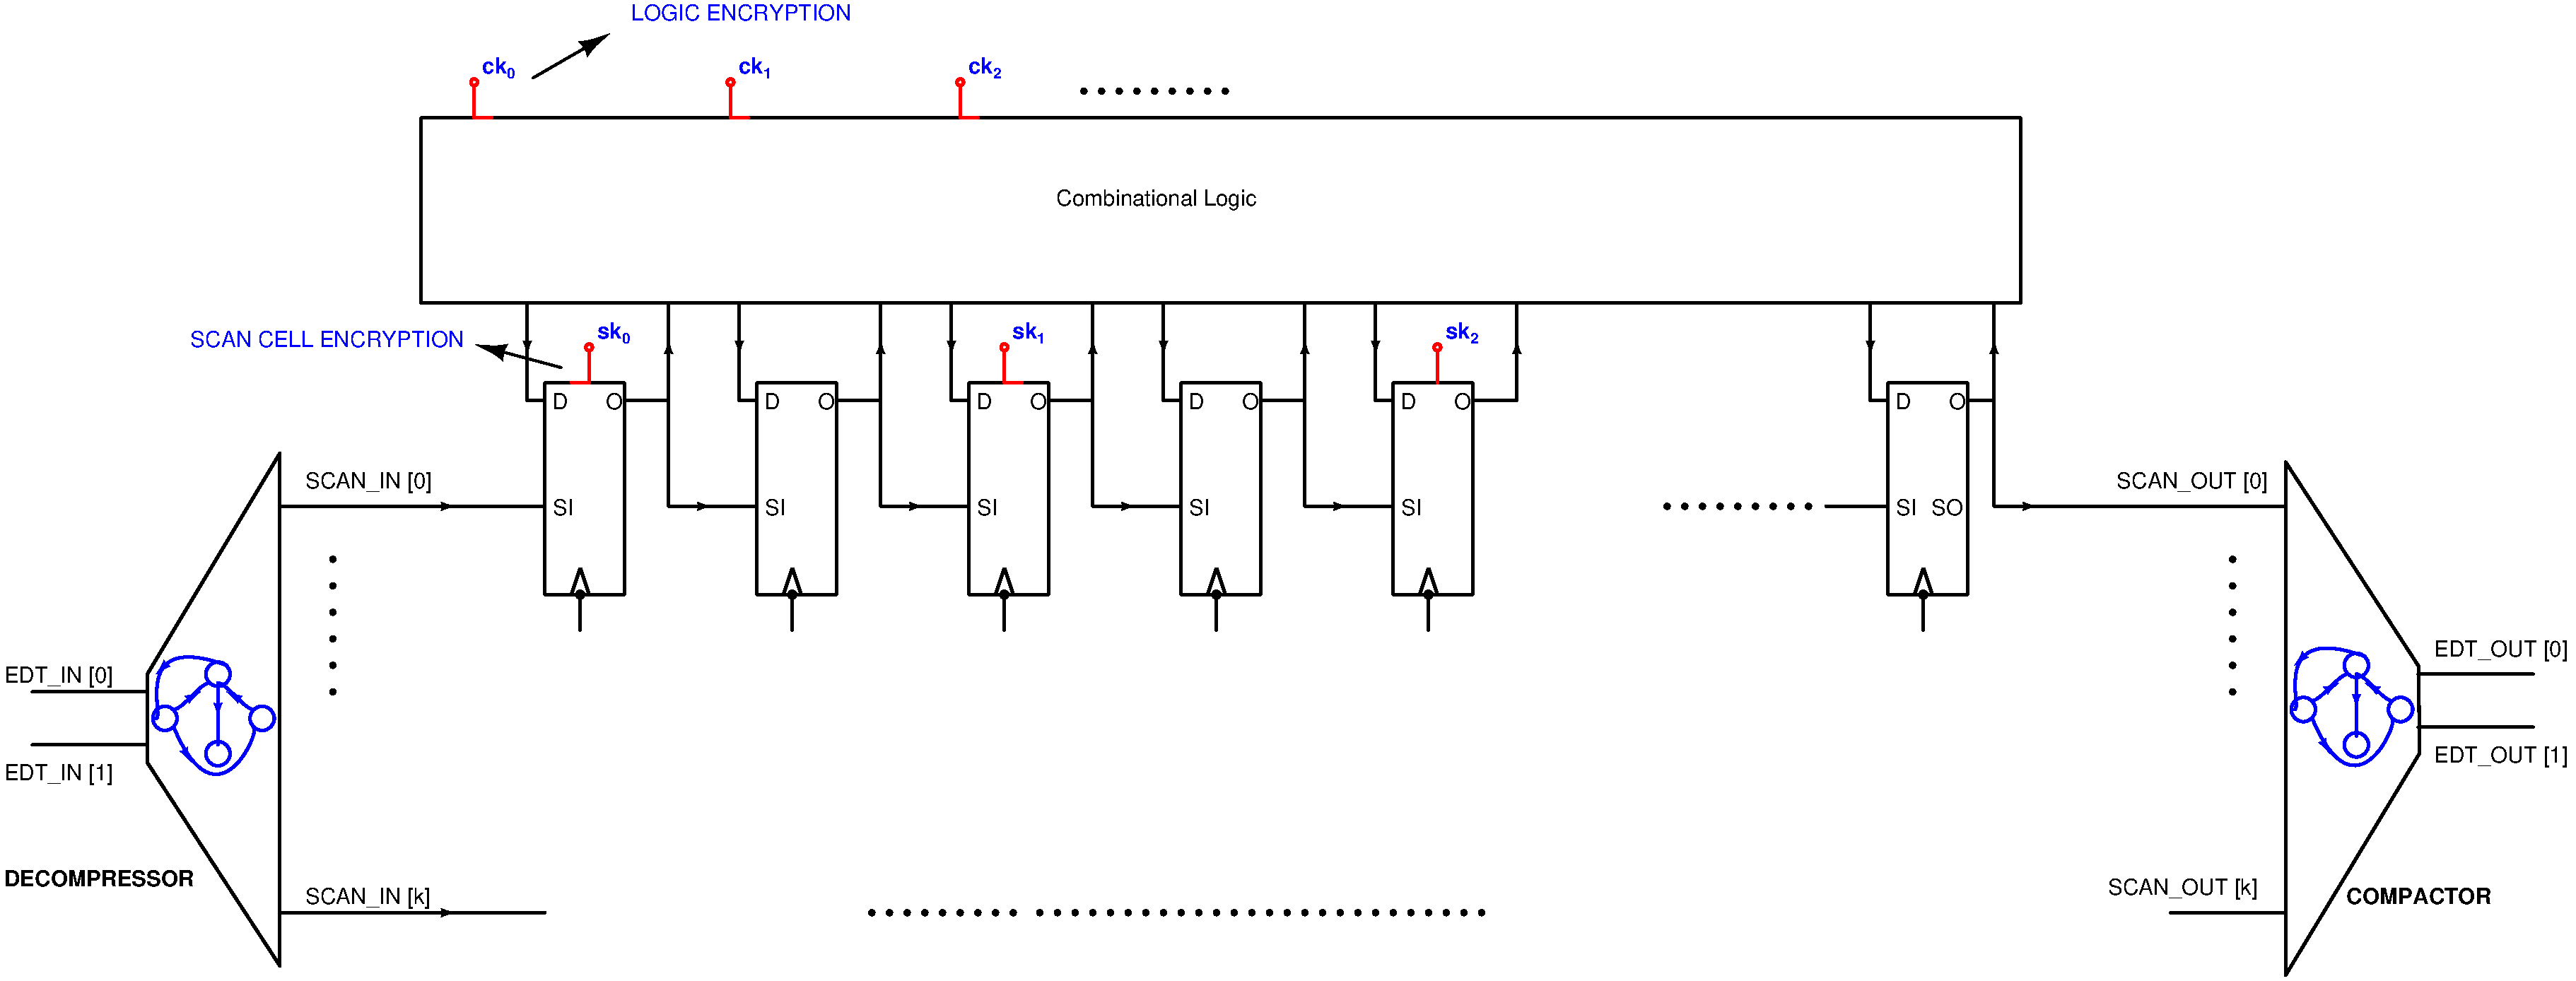
\includegraphics[scale=0.14]{fig/encrypted-DFT.pdf}
\caption{DFT Encryption}
\label{fig:encrypted-DFT}
\end{figure}


\begin{figure}
\centering
\includegraphics[scale=0.6]{fig/occ.pdf}
\caption{On-chip clock control}
\label{fig:occ}
\end{figure}


Figure~\ref{fig:encrypted-DFT} shows the encrypted design-for-testability (DFT) architecture, where both the combinational logic and flip-flops are encrypted, while the decompressor/compactor are unencrypted. 
Hence, the decompressor and compactor should be bypassed, to directly access the scan chains. Figure~\ref{fig:occ} shows the on-chip clock control scheme used in modern SoCs. The attacker places the IC in scan mode of operation by asserting $TEST\_MODE$ signal shown in this figure. To apply the desired input vector to the combinational portion of the IC, the attacker assigns the flip-flops to desired values by placing the IC in scan-shift mode, by further asserting $SCAN\_EN$ signal. After initialization, the $SCAN\_EN$ signal is deasserted and $SLOW\_CLK$ is pulsed, to capture the response back into the flip-flops. The $SCAN\_EN$ signal is asserted again to read-out the captured response is read-out, while parallelly reading-in next attack vector. The attacker repeats this procedure until all distinguishing input patterns are applied to the IC. 

%\section{Motivation}

Figure~\ref{fig:c432-logic-encrypted-observe-flops} shows the implementation of a logic-encrypted version of \texttt{c432} circuit, with observe flip-flops at the primary outputs.  
\begin{figure}[!htbp]
	\centering
	\includegraphics[scale=0.3]{fig/c432-sequential}
	\caption{Logic encrypted \texttt{c432} circuit, with observe flip-flops}
	\label{fig:c432-logic-encrypted-observe-flops}
\end{figure}


\input{proposed-sequential-locking}
\section{Results}

%\noindent Results of using the encrypted flip-flop proposed in~\cite{rajit:encryptFF}, as well as the proposed encrypted flip-flop are shown in Table~\ref{tab:results-proposed-eff}. 
\begin{table*}[!htbp]
\begin{center}
\caption{Success in Functional Output Corruption}
\label{tab:results-proposed-eff}
\begin{tabular}{|c|c|c|c|c|c|c|c|c|c|c|}
\hline
Bench. & \multicolumn{2}{c|}{RND (5\%)} & \multicolumn{2}{c|}{DAC12 (5\%)} & \multicolumn{2}{c|}{IOLTS14 (5\%)} & \multicolumn{2}{c|}{TOC13'XOR (5\%)} & \multicolumn{2}{c|}{TOC13'MUX (5\%)} \\
\hline
       &ScanSAT~\cite{lilas:aspdac19}  & Proposed &ScanSAT~\cite{lilas:aspdac19} & Proposed &ScanSAT~\cite{lilas:aspdac19} & Proposed &ScanSAT~\cite{lilas:aspdac19} & Proposed &ScanSAT~\cite{lilas:aspdac19} & Proposed  \\
%\hline
%       &~\cite{dupuis:iolts14}  & $P_1$  & $P_2$ &~\cite{dupuis:iolts14}  & $P_1$ & $P_2$ &~\cite{dupuis:iolts14}  & $P_1$ & $P_2$ &~\cite{dupuis:iolts14}  & $P_1$ & $P_2$ &~\cite{dupuis:iolts14}  & $P_1$ & $P_2$  \\
\hline 
apex2      &\redx	&\greencheck		&\redx &\redx			&\redx &\greencheck 		&\greencheck &\greencheck			&\redx &\greencheck \\
\hline 
i4       &\greencheck &\greencheck 		&\redx &\greencheck		&\redx &\greencheck 	&\greencheck &\greencheck			&\redx &\greencheck \\
\hline 
c432    &\redx &\greencheck 			&\redx &\greencheck		&\redx &\greencheck  	&\redx &\greencheck 				&\redx &\greencheck  \\
\hline 
ex1010  &\greencheck &\greencheck 		&\redx &\greencheck		&\redx &\greencheck 	&\greencheck &\greencheck			&\redx &\greencheck \\
\hline
dalu    &\greencheck	&\greencheck		&\redx &\greencheck		&\redx &\greencheck 	&\greencheck &\greencheck			&\redx &\greencheck \\
\hline  
apex4   &\redx	&\greencheck			&\redx &\greencheck		&\redx &\greencheck 	&\greencheck &\greencheck			&\greencheck &\greencheck \\
\hline 
c3540   &\greencheck &\greencheck 		&\redx &\greencheck		&\redx &\greencheck	&\redx &\greencheck				&\redx &\greencheck \\
\hline
c1908   &\greencheck &\greencheck		&\redx &\greencheck		&\redx &\greencheck 	&\redx &\greencheck 				&\redx &\greencheck \\
\hline 
c880    &\greencheck	&\greencheck		&\greencheck &\greencheck	&\redx &\greencheck 	&\redx &\greencheck 				&\redx &\greencheck \\
\hline 
c1355   &\greencheck &\greencheck		&\redx &\greencheck		&\redx &\greencheck 	&\greencheck &\greencheck			&\redx &\greencheck \\
\hline 
c499    &\redx &\greencheck 			&\redx &\greencheck 		&\redx &\greencheck 	&\redx &\greencheck				&\redx &\greencheck \\
\hline 
seq     &\greencheck &\greencheck		&\redx &\greencheck		&\redx &\greencheck 	&\greencheck &\greencheck			&\redx &\greencheck \\
\hline 
k2     	&\greencheck &\greencheck		&\redx &\greencheck		&\redx &\greencheck	&\greencheck &\greencheck			&\redx &\greencheck \\
\hline 
ex5     &\greencheck &\greencheck		&\redx &\greencheck		&\redx &\greencheck 	&\greencheck &\greencheck			&\redx &\greencheck \\
\hline 
i9     	&\greencheck &\greencheck		&\redx &\greencheck		&\redx &\greencheck 	&\redx &\greencheck				&\redx &\greencheck \\
\hline 
i7      &\greencheck &\greencheck 		&\redx &\greencheck		&\redx &\greencheck 	&\greencheck &\greencheck			&\redx &\greencheck \\
\hline 
i8     	&\greencheck &\greencheck		&\redx &\greencheck		&\redx &\greencheck 	&\greencheck &\greencheck			&\redx &\greencheck \\
\hline 
c7552   &\greencheck &\greencheck		&\redx &\greencheck		&\redx &\greencheck 	&\greencheck &\greencheck			&\redx &\greencheck \\
\hline 
c5315   &\greencheck &\greencheck		&\greencheck &\greencheck	&\redx &\greencheck 	&\greencheck &\greencheck			&\redx &\greencheck \\
%\hline 
%c2670  &\greencheck &\greencheck		&- &-				&\redx &\greencheck	& &\greencheck &\greencheck 			&\redx &\greencheck \\
\hline 
des     &\greencheck &\greencheck 		&\redx &\greencheck		&\redx &\greencheck 	&\greencheck &\greencheck			&\redx &\greencheck \\
\hline 
Success rate  &$80\%$ &$100\%$			&$10\%$ &$95\%$			&$0\%$ &$100\%$ 		&$70\%$ &$100\%$				&$5\%$ &$100\%$ \\
\hline 
\end{tabular}
\end{center}
\end{table*}

\begin{table*}[!htbp]
\begin{center}
\caption{Increase in Decryption Time}
\label{tab:results-RT-proposed-eff}
\begin{tabular}{|c|c|c|c|c|c|c|c|c|c|c|c|c|c|c|c|c|}
\hline
Ben. & \#POs & \multicolumn{3}{c|}{RND~\cite{farinaz:epic}} & \multicolumn{3}{c|}{DAC12~\cite{jv:dac12}} & \multicolumn{3}{c|}{IOLTS14~\cite{dupuis:iolts14}} & \multicolumn{3}{c|}{TOC13'XOR~\cite{jv:tc15}} & \multicolumn{3}{c|}{TOC13'MUX~\cite{jv:tc15}} \\
\hline
	&    & ~\cite{dupuis:iolts14} & Prop. &Inc. & ~\cite{dupuis:iolts14} & Prop. &Inc. & ~\cite{dupuis:iolts14} & Prop. &Inc. & ~\cite{dupuis:iolts14} & Prop. &Inc. &~\cite{dupuis:iolts14} & Prop. &Inc. \\
\hline 
apex2   &3   &0.18s &0.26s &		&0.13s &0.75s &$5.8\times$		&0.05s &0.05s &$1 \times$ 		&0.14s & &			&0.38s &0.07s &$0.2 \times$ \\
\hline 
i4      &6	&0.05s & &		&0.05s &0.08s &$1.6\times$		&0.03s &0.07s &$2.3 \times$ 		&0.11s & &			&0.04s &0.07s &$1.8 \times$ \\
\hline 
c432    &7   &0.02s &0.04s &$2\times$	&0.02s &0.04s &$2\times$ 		&0.03s &0.04s &$1.3 \times$  		&0.04s &0.07s & 			&0.03s &0.04s &$1.3 \times$  \\
\hline 
ex1010  &10   	&7.44s & &		&13.6s &16.6s &$1.2\times$		&1.20s &3.49s &$2.9 \times$ 		&23.75s & &			&3.48s &5.45s &$1.6 \times$ \\
\hline 
dalu   &16    &1.74s & &		&2.35s &5.8s &$2.5\times$		&0.31s &7.67s &$24.7 \times$ 		&49.59s & &			&1.15s &7.47s &$6.5 \times$ \\
\hline 
apex4   &19   &5.2s &14.6s &		&19.8s &24s &$1.2\times$			&0.75s &3.04s &$4.1 \times$ 		&53.47s & &			&6.21s &25.37s &$4.1 \times$ \\
\hline 
c3540   &22   	&1.94s & &		&4.87s &11.9s &$2.4\times$		&0.26s &0.34s &$1.3 \times$ 		&2.30s &3.86s &			&2.63s &3.10s &$1.2 \times$ \\
\hline 
c1908   &25   &0.54s & &		&0.88s &4.6s &$5.2\times$		&0.33s &1.54s &$4.7 \times$ 		&19.25s &12.01s &			&0.18s &1.60s &$8.9 \times$ \\
\hline 
c880    &26    &0.14s	& &		&0.13s &0.89s &$6.9\times$		&0.07s &1.14s &$16.3 \times$ 		&0.59s &3.96s &			&0.10s &1.81s &$18.1 \times$ \\
\hline 
c1355    &32  	 &3.75s & &		&0.39s &3.6s &$9.2\times$		&0.05s &0.83s &$16.6 \times$ 		&26.05s & &			&0.13s &2.53s &$19.5 \times$ \\
\hline 	
c499    &32  &0.13s &2.72s & 		&0.27s &3.2s &11.9$\times$			&1.13s &1.41s &$1.3 \times$ 		&0.27s &1.25s &			&0.09s &2.72s &$30.2 \times$ \\
\hline 
seq     &35 	&3.6s & &		&5.8s &6.2s &$1.1\times$		&1.82s &3.27s &$1.8 \times$ 		&281s & &			&3.22s &16.96s &$5.3 \times$ \\
\hline 
k2      &45	&2.6s & &		&2.37s &17.8s &$7.5\times$		&0.34s &9.24s &$27.2 \times$ 		&3.29s & &			&0.49s &6.40s &$13.1 \times$ \\
\hline 
ex5    &63 	&1.68s & &		&0.69s &36.1s &$52.3\times$		&8.6s &174s &$20.2 \times$ 		&6.99s & &			&1.88s &6.52s &$3.5 \times$ \\
\hline
i9      &63	&2.6s & &		&1.1s &26.1s &$23.7\times$		&0.29s &16.7s &$57.6 \times$ 		&1.56s &23.27s &			&0.78s &17.81s &$22.8 \times$ \\
\hline 
i7      &67	&2.68s & &		&1.02s &13.6s &$13.3\times$		&0.11s &5.64s &$51.3 \times$ 		&185s & &			&0.52s &3.01s &$5.8 \times$ \\
\hline 
i8      &81	&7.37s & &		&7.6s &79.7s &$10.5\times$		&0.22s &8.18s &$37.2 \times$ 		&8.84s & &			&2.40s &3.69s &$1.5 \times$ \\
\hline 
c7552   &108   	&11.7s & &		&50.5s & 1 hr &$71.3\times$		&3.20s &27.3s &$8.5 \times$ 		& & &			&5.48s &$\approx$ 11 hrs. &$7226 \times$ \\
\hline 
c5315   &123   	&12.2s & &		&14.4s &146s &$10.1\times$		&4.64s &515s &$111 \times$ 		&714s & &			&2.91s &62.79s &$21.6 \times$ \\
%\hline 
%c2670   &140	&3.29s & &		& - & - & -				&2.02s &34.52s &$17.1 \times$		& & & 			&1.01s &1.03s &$1.02 \times$ \\
\hline 
des     &245	&66.6s & &		&408s &2668s &6.5$\times$		&2.52s &375s &$149 \times$ 		&67.0s &3247s &			&24.97s &$\approx$ 2 hrs. &$288.4 \times$ \\
\hline 
\end{tabular}
\end{center}
\end{table*}


\noindent Running time comparisons are shown in Figure~\ref{fig:running-time-comparison-all}. 
\begin{figure*}[]
\centering
\begin{tikzpicture}
\centering
\begin{semilogyaxis}[
height=9cm,
width=1.5\columnwidth,
enlargelimits=-0.1,
y tick label style={/pgf/number format/fixed},
x tick label style={/pgf/number format/fixed},
ymax=40000.00,
ymin=0.00,
xmax=20.00,
xmin=1.00,
grid=major,
%legend style={at={(0.50,1.2)},anchor=north,legend columns=4,draw=none,fill=none},
legend style={at={(0.8,0.8)},anchor=south east,legend columns=2,fill=none},
ylabel={$Time\ to\ Solve(s)$},
xlabel={$\#\ of\ decrypted\ circuits$},
]
\addplot [dashed, mark=o,mark size=3.0,line width = 1.0, color=blue!70!white] table[x index = 0,y index =1]{data_file_dac12_iolts14_toc13mux.txt};
\addplot [mark=o,mark size=3.0,line width = 1.0,color=red!70!white] table[x index = 0,y index =2]{data_file_dac12_iolts14_toc13mux.txt};
\addplot [dashed, mark=*,mark size=3.0,line width = 1.0, color=blue!70!white] table[x index = 0,y index =3]{data_file_dac12_iolts14_toc13mux.txt};
\addplot [mark=*,mark size=3.0,line width = 1.0,color=red!70!white] table[x index = 0,y index =4]{data_file_dac12_iolts14_toc13mux.txt};
\addplot [dashed, mark=triangle*,mark size=3.0,line width = 1.0, color=blue!70!white] table[x index = 0,y index =5]{data_file_dac12_iolts14_toc13mux.txt};
\addplot [mark=triangle*,mark size=3.0,line width = 1.0,color=red!70!white] table[x index = 0,y index =6]{data_file_dac12_iolts14_toc13mux.txt};
\legend{$ScanSAT-DAC12$, $Proposed-DAC12$, $ScanSAT-IOLTS14$, $Proposed-IOLTS14$, $ScanSAT-TOC13MUX$, $Proposed-TOC13MUX$}
\end{semilogyaxis}
\end{tikzpicture}
\caption{Running Time Comparisons}
\label{fig:running-time-comparison-all}
\end{figure*}



\bibliographystyle{ieeetr}
\bibliography{refs}

%\section{Acknowledgement}
\end{document}

